%------------------------------------------------------------
%------------------------------------------------------------
\section{The {\UTP} language}
\label{sec:schema}
The {\UTP} language splits the representation of a timetabling instance into three syntactic components, namely, an entity model, a rules set and a solution. 
We do not present here the {\XML} syntax and {\JSON} format used for encoding (see \cite{USPsite} for details).
Rather, we provide an informal description of the components 
and the type of features and requirements that may be factored in.
We also provide set-theoretic semantics for the rules language and flattening process
and present the catalog of {\UTP} predicates.

%motivate design choices, 
%and highlight differences with related work.

%The entity model defines the schedule horizon, courses and resources of the instance and encodes core %domain and cardinality %compatibility, capacity and flow % distribution
%constraints relating to session scheduling, resource allocation, and student sectioning.
%Rules express additional constraints meant to capture stakeholder requirements on particular aspects of the problem.
%To this end, the schema provides a catalog of timetabling-specific constraint predicates and embeds a rules language to apply predicates on chosen entities.
%The solution component includes a list of choices made for some or all of the decisions at stake (e.g., start time of a session).
%Note that rules set and solution components may be omitted. 
%% Besides, the listed solution is not required to be consistent with the constraints enforced by the entity model or the rules set.
%% This allows to tackle subproblems using separate instances and to support timetable generation or repair tasks.


% Each rule is an intensional representation of a collection of constraints applying to different entities.
% {\UTP} instances may thus be compiled to lower-level representations that explicitly declare all constraints and whose format is compatible with {\CP} languages.
%{\UTP} instances may therefore be compiled into lower-level representations that lists all constraints and whose format is tailored to back-end solvers.

%------------------------------------------------------------
%------------------------------------------------------------

\begin{figure*}[!ht]
\centering
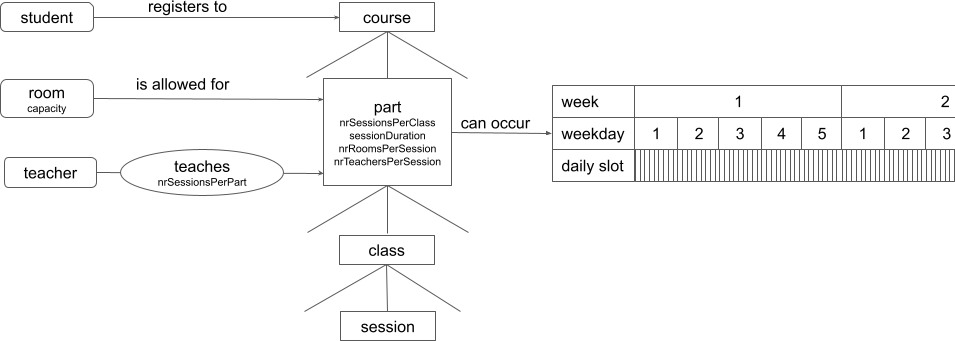
\includegraphics[width=.85\textwidth]{img/utp_entity_model.png}
\caption{Entity model}
\label{fig:utp-entity-model}
\end{figure*}

\subsection{Entity model}
\label{sec:entity-model}
The entity model of a {\UTP} instance defines its schedule horizon, course structure and resources, as well as the properties of entities and the relational maps (see Figure~\ref{fig:utp-entity-model}).  
First, the model uses a time grid that decomposes into weeks, weekdays and daily slots, % (see Figure~\ref{fig:utp-time-grid}),
the number of which is instance-specific.
Weeks share the same weekdays and weekdays the same daily slots.
The latter make up 24 hours and have the same duration (e.g. 24 daily slots will represent 1 hour each, 1440 daily slots represent 1 minute each).
%\marc{C'est pas forcément mesuré en minutes ... Dans nos exemples oui, mais justement c'est custom.
%Il faudrait dire "The latter makes up 24 hours and have the same duration, meaning that 3 dailyslots will represent 8 hours each, or 1440 dailyslots represent 1 minute each." ?}
Note that neither successive weeks nor successive weekdays are assumed to be consecutive.
The schedule horizon is implicitly defined by the series of time slots mapping to week, weekday and daily slot combinations.
Slots hence serve as time points to represent start and end times of course sessions and to measure durations (session length, travel times).

% % For one-column wide figures use
% \begin{figure}[h]
% % \includegraphics{utp-time-grid.eps}
% \caption{{\UTP} 3-layered time grid}
% \label{fig:utp-time-grid}
% \end{figure}

Courses have a tree-structure wherein each course (i.e., course topics) decomposes into parts (lecture, practical work \ldots), parts into classes, and classes into sessions.
Class sessions are the elementary tasks to schedule when solving a {\UTP} instance
and the model fixes their number, duration and sequencing.
On the one hand, the classes of a course part are decomposed into an identical number of sessions of equal duration, both constants being part-specific.
Although this approach forbids alternative class decompositions using variable session durations, 
it %provides flexibility for handling sessions independently wrt. scheduling and resource allocation.
%Fixed decompositions also 
facilitates the formulation of requirements which depend on clear-cut sessions (e.g., planning parallel sessions ``mid-way'' through a course).
On the other hand, the model requires that the sessions of a class be ranked and sequenced accordingly in any solution.
Note that sessions are considered uninterruptible and, in particular, may not overlap two days. 

{\UTP} resources fall into 3 types, namely, rooms, teachers, students (gathered into groups).
All the resources of an instance are declared and typed in the entity model.
In practice, various restrictions resulting from upstream processes apply on the resourcing and timing of courses.
Basic restrictions come in the form of compatibility constraints that list the suitable rooms, eligible teachers, candidate students and allowed times for the different courses 
(e.g., faculties prescribing degree-specific time grids, departments implementing room pooling policies, %alternative 
teachers applying for courses, student registrations). %registering to courses).
Such constraints are built in the entity model but scoped differently depending on resource types.
Specifically, each course part is assigned sets of possible start times, rooms and teachers which propagate automatically to all its sessions.
As for students, course registrations are listed separately and %the possible students for a session are those registered to the course it sits in.
any student registered to a course is considered a possible candidate for each of its sessions.

Beyond plain compatibility, resource utilization is subject to demand and capacity constraints.
Since modalities differ from one environment to the next, the language supports both disjunctive and cumulative resources as well single- and multi-resource sessions. 
Students, teachers or rooms qualify as cumulative resources if they 
can attend, teach or host simultaneous sessions. %, respectively.
Cumulative resources are paramount to meet flexible attendance requirements (e.g., students assigned optional tutoring sessions that may overlap with mandatory courses) or to handle multi-class events (e.g., rooms hosting joint exam or conference sessions).
The schema assumes no limit on the number of parallel sessions teachers and students may attend.
Rooms however may only host class sessions whose cumulated headcount
is within their capacity.
Upper bounds on room capacity and class size are encoded for all rooms and classes in the entity model with the possibility to leave room capacity unbounded (e.g., virtual rooms). 
Note that all resources default to cumulative resources but this assumption may be overridden using disjunctive rules on a per resource basis.
% a {\UTP} instance may freely mix disjunctive and cumulative resources. 

A multi-resource session is a session requiring multiple resources of the same type. %at any point in time.
The need for sessions using multiple rooms or teachers arises in many practical situations (e.g., multi-room sessions for hybrid teaching, joint supervision of practical work sessions, exams requiring several adjudicators).
The number of resources required per session is typically fixed on course parts and  
such restrictions are expressed in the entity model through cardinality constraints. %that are lifted to course parts. 
Specifically, each course part indicates the number of teachers required per session 
and whether its sessions are single- or multi-rooms.
Multi-room sessions impose specific constraints:
allocated rooms are disjunctive for the time of the session only and their total capacity is considered for hosting the students attending the session.
Note that the model allows for sessions without teachers or rooms (e.g., unsupervised student projects). 
%a {\UTP} instance may freely mix single- and multi-resource sessions as well as disjunctive and cumulative resources. 

The entity model also encodes flow constraints that govern the distribution of students and teachers over courses. 
These constraints %relating to the distribution of students and teachers over courses 
are usually elicited ahead of scheduling during registration and capacity planning stages (e.g., departments distributing session volumes among designated teachers). 
As mentioned above, students only register for courses, not for classes nor sessions, and solving a {\UTP} instance involves determining student-to-class assignments that are consistent with the course structure.
Specifically, every student must be assigned a single class in each part of a course he has registered to and must attend all sessions of these classes. 
Group nesting constraints may also be stated between classes %. %to enforce equality or set inclusion relations between their sets of participants.
%These constraints serve 
to implement course-specific or cross-course sectioning policies (e.g., aggregating student groups bottom-up from practicals to lectures, enforcing identical groups between classes of different courses of a curriculum).
As for staff distribution, each teacher is assigned a fixed volume of sessions in each course part he is eligible for, leaving teacher-to-session assignment decisions to solvers.

Note finally that the language provides the ability to label entities and define custom classes of elements (e.g., teams of teachers, blocks of rooms). %that complement the built-in types. 
%Entities sharing the same label form a type of their own named after the label.
Labels complement built-in types and entity identifiers as a means to select entities within rules.
  


%Rules may then help to enforce instance-specific scheduling or resource allocation constraints on any entity or group of entities, e.g. casting a problem instance as a pure disjunctive scheduling problem.

%First, teachers are explicitly represented on par with rooms. Student groups may optionally be modelled too to cater for workflows where student sectioning is performed ahead of session scheduling. 

%The {\UTP} schema also differs on the way sessions are time-framed in a class. Indeed a class' sessions are just chronologically ranked and specific scheduling requirements are enforced per class (e.g., periodicity) or across classes (e.g., simultaneity) through explicit rules.
%while leaving the opportunity to jointly state and solve both problems. Second, it represents teachers explicitly, allows for class sessions requiring multiple resources (e.g., multi-room or -teacher sessions),
%and supports resource distribution constraints (e.g., eligible teachers and their workload per course part measured in sessions).
%and rooms %(including virtual rooms) 


We formalize below the entity model and introduce notations that will be used thereafter.
Let ${\ENTITY}$ denote the set of entities
and ${\SESSION}$ the set of sessions.
${\ENTITY}$ is partitioned into   
a set of courses ${\COURSE}$, 
a set of course parts ${\PART}$, 
a set of classes ${\CLASS}$, 
a set of students ${\STUDENT}$, 
a set of teachers ${\TEACHER}$,
a set of rooms ${\ROOM}$,
and the singleton domain of courses ${\COURSES}$ 
(${\COURSES}=\myset{\COURSE}$). 
Let 
%${\COURSES}$ denote the course domain, 
%${\COURSE}$ the set of courses (${\COURSES}=\myset{\COURSE}$), 
%${\PART}$ the set of course parts, 
%${\CLASS}$ the set of classes, 
%${\SESSION}$ the set of sessions, 
%${\STUDENT}$ the set of students, 
%${\TEACHER}$ the set of teachers, 
%and 
%${\ROOM}$ the set of rooms.
$
{\TYPE}
=
\myset{
{\COURSES}, 
{\COURSE},
{\PART},
{\CLASS},
{\STUDENT},
{\TEACHER},
{\ROOM}
}
$
denote the set of entity types
(${\ENTITY}=\setunion{X}{\TYPE}{X}$)
and 
$
{\prec}
=
\myset{
({\COURSES},{\COURSE}),
({\COURSE},{\PART}),
({\PART},{\CLASS}),
({\CLASS},{\SESSION}),
({\STUDENT},{\COURSE}),
({\TEACHER},{\PART}),
({\ROOM},{\PART})
}
$
denote the relation over 
${\TYPE}\cup\myset{\SESSION}$ 
that models the course hierarchy
and the distribution of resource types over course components.
${\prec^{*}}$
%${\preceq^{*}}$
denotes the transitive %and reflexive 
closure of
${\prec}$ 
over
${\TYPE}\cup\myset{\SESSION}$
and
${\maptype{X}{Y}}:X\rightarrow2^{Y}$
denotes the function mapping each element of $X$ to its set of compatible elements in $Y$
for each pair %$(X,Y)$ such that 
%$X{\preceq^{*}}Y$.
$X{\prec^{*}}Y$.
For instance, 
${\maptype{\STUDENT}{\COURSE}}$ 
represents the distribution of students over courses, 
${\maptype{\COURSE}{\PART}}$ 
the decomposition of courses into course parts,
and ${\maptype{\STUDENT}{\PART}}$ 
the inferred distribution of students over course parts.
The functions corresponding to the pairs of $\prec$
are directly encoded in the entity model
and the remaining functions are defined inductively using recursive aggregation. 
Rule (\ref{model:hierarchy}) below models the hierarchical decomposition of course elements\footnote{$\sqcup$ denotes the disjoint union operation, i.e. set union over pairwise disjoint sets.}
and
Rule (\ref{model:transitivity}) is the closure rule over 
%$\preceq^{*}$. 
$\prec^{*}$. 
%Rule (\ref{model:symmetry}) enforces symmetry over all compatible pairs,
%and Rule (\ref{model:selfmap}) completes the model with self-maps. 

%\todo[inline]{i en indice dans les équations suivantes, formulation non expliquée. $d_i$ serait l'ensemble des couples (a,b) de la relation tels que a=i ?}
%\vincent{Dans ce cas, comme d est une fonction, ça serait plutôt $d^{Y,Z}(i)$}
%\marc{On en discutait avec DG et effectivement c'est ce qu'on a conclu. Cependant, plus tard cette notation est réutilisée avec en indice des ensembles de valeurs. Il faut donc faire attention à bien introduire cette notation.
%De plus je rajouterais une petite remarque : $\forall (X,Y)$ et non $\forall X,Y$ ?}

\begin{multline}
\forall (X,Y) \in  \myset{ ({\COURSES},{\COURSE}), ({\COURSE},{\PART}), ({\PART},{\CLASS}), ({\CLASS},{\SESSION}) }: \\
Y=\setpartition{i}{X}{\map{X}{Y}{i}} \label{model:hierarchy}
\end{multline}
\begin{multline}
\forall X,Y,Z \in {\TYPE}\cup\myset{\SESSION}:\\
\mbox{\hspace{-10em}}X\preceq^{*} Y\preceq^{*} Z 
\Rightarrow \\
(\forall i \in X:
\map{X}{Z}{i}=\setpartition{j}{\map{X}{Y}{i}}{\map{Y}{Z}{j}}
 \label{model:transitivity})
%%
%%\forall X,Y \in {\TYPE}:
%%X\preceq^{*} Y 
%%\Rightarrow 
%%(\forall i \in X, j \in Y:
%%j \in \domarg{X}{Y}{i} \Leftrightarrow i \in \domarg{Y}{X}{j}
%%) \label{model:symmetry}\\
%%
%\forall X \in {\TYPE}\cup\myset{\SESSION},
%i \in X:
%\domarg{X}{X}{i} = \myset{i} \label{model:selfmap}
%%
\end{multline}

%We shall denote by
%${\RANK}$
%the range of session ranks,
%${\maptype{\RANK}{\SESSION}}:\RANK\rightarrow2{^\SESSION}$
%the rank-based partitioning of sessions,
%and
%${\LABEL}$
%the set of labels 
%(${\LABEL}\subseteq2^{{\ENTITY}}$)
%completed 
%with the whole set of entities %to mock label optionality
%($\ENTITY\in{\LABEL}$)
%and singleton entities %to support identity-based selection
%($\myset{\myset{e}\ |\ e\in{\ENTITY}}\subseteq{\LABEL}$).
%As discussed in section~\ref{sec:rules},
%labels are optional filters used in rules to select entities
%hence the formal inclusion of $\ENTITY$ in ${\LABEL}$ to mock label optionality.
%Likewise, entity identifiers are used as an alternative to labels
%hence the inclusion of singleton entities in ${\LABEL}$.

%------------------------------------------------------------
%------------------------------------------------------------
\subsection{Predicates and constraints}
\label{sec:constraints}
{\UTP} constraints apply to pairs, called e-maps, which associate an entity with a non-empty subset of its compatible sessions.
%which we call e-maps. 
Constraints are built with predicates whose signature includes e-map variables%ranging over the set of e-maps
, the number of which is referred to as the arity of the predicate. 
Note that some predicates may also accept parameters.
Let 
${\EMAP}=
\setunion{X}{\TYPE}
\myset{(e,S')\ |\ e\in X,S'\subseteq\map{X}{\SESSION}{e}\wedge S'\neq\emptyset}$
denote the set of e-maps,
a {\UTP} constraint has the form
\begin{align}
c((e_1,S_1),\ldots,(e_m,S_m),p_1,\ldots,p_n) \label{rule:constraint}
\end{align}
where 
$c$ is a predicate symbol of arity $m$,
$(e_1,S_1)$, $\ldots$, $(e_m,S_m)$ are e-maps ($(e_i,S_i)\in{\EMAP}$, $i=1\ldots m$) 
and 
$p_1,\ldots,p_n$ are values for the parameters of $c$ ($n\geq0$).


Every predicate may be used indistinctly with e-maps defined on course elements or on resources.
E-maps defined on resources are interpreted as conditional session-to-resource assignments
when checking constraints 
whereas e-maps defined on course elements are unconditional assignments since they model constitutive sessions.
In other words, 
a constraint is only evaluated
on the sessions whose assignments in the considered solution are consistent with its e-map arguments.\footnote{Formally, let $\var{E}{\SESSION}{e}$ be the variable denoting the set of sessions assigned to entity $e$ and $S'_1,\ldots,S'_m$ be sets of sessions, the conditionality of a constraint $c$ is stated as follows: 
$(\var{E}{\SESSION}{e_1}=S'_1 \wedge \var{E}{\SESSION}{e_m}=S'_m)
\Rightarrow
(c((e_1,S_1),\ldots,(e_m,S_m),p_1,\ldots,p_n)
\Leftrightarrow
c((e_1,S_1\cap S'_1),\ldots,(e_m,S_m\cap S'_m),p_1,\ldots,p_n))$.
}
It follows that 
a constraint is evaluated on every session that is mapped to a course element.
In particular, constraints that apply exclusively to course elements are unconditional. 
Note also that the use of e-maps that model the whole set of sessions compatible with an entity 
will necessarily constrain any session that may be assigned to this entity.


%Every predicate may be used indistinctly with e-maps defined on course elements or on resources which we call c-maps and r-maps, respectively. R-maps are interpreted conditionally since they map a resource to some of its possible sessions whereas c-maps model unconditional assignments since they model constitutive sessions of course elements. In other words, a constraint must be evaluated on every session of every c-map in its scope but only on the sessions of its r-maps whose resource assignment is compatible with the proposed solution.\footnote{Formally, let $\var{E}{\SESSION}{e}$ be the variable denoting the set of sessions assigned to entity $e$ and $S'_1,\ldots,S'_m$ be sets of sessions, the conditionality of a constraint $c$ is stated as follows:  $(\var{E}{\SESSION}{e_1}=S'_1 \wedge \var{E}{\SESSION}{e_m}=S'_m) \Rightarrow (c((e_1,S_1),\ldots,(e_m,S_m),p_1,\ldots,p_n) \Leftrightarrow c((e_1,S_1\cap S'_1),\ldots,(e_m,S_m\cap S'_m),p_1,\ldots,p_n))$.}
%effectively assigns to the resource of the r-map.
%(see Rule (\ref{rule:conditionality})).
%It follows that constraints applying exclusively to c-maps are unconditional. Besides, the scoping of e-maps that model the whole set of sessions compatible with an entity will constrain every session assigned to a resource or constitutive of a course element.
%%The rule below %(\ref{rule:conditionality}) models the conditionality of constraints.

%{\footnotesize{
%\begin{multline}
%\forall S'_1,\ldots,S'_m\in{\SESSION}:
%(\var{E}{\SESSION}{e_1}=S'_1 \wedge \var{E}{\SESSION}{e_m}=S'_m)
%\Rightarrow\\
%(c((e_1,S_1),\ldots,(e_m,S_m),p_1,\ldots,p_n)
%\Leftrightarrow
%c((e_1,S_1\cap S'_1),\ldots,(e_m,S_m\cap S'_m),p_1,\ldots,p_n))
%\label{rule:conditionality}
%\end{multline}
%}}

\begin{table*}[!ht]
\resizebox{\textwidth}{!}{%
\centering
\begin{tabular}{|l|l|l|l|}
\hline
\textbf{Name}               & \textbf{Arity} & \textbf{Parametric} & \textbf{Semantics}\\ \hline

%assign\_slot               & 1         & yes   & Assign a slot or slot tuple to a session\\ \hline
%assign\_room               & 1         & yes   & Assign a set of room to session in entry\\ \hline

%allocation\_group           & 1        & no    & Domain allocation for class with group in the solution\\ \hline
%part\_schedule              & 1        & no    & Allowed start time slots for sessions\\ \hline
%domain\_class\_group        & 1        & no    & Allowed groups for classes (solution input)\\ \hline
%domain\_session\_teacher    & 1        & no    & Allowed teachers for sessions\\ \hline
%domain\_class\_room         & 1        & no    & Allowed rooms for sessions\\ \hline

{\SAMEDAILYSLOT}            & 1         & no    & Sessions start on the same daily slot\\ \hline
{\SAMEWEEKDAY}              & 1         & no    & Sessions start on the same weekday\\ \hline
{\SAMEWEEKLYSLOT}           & 1         & no    & Sessions start on the same weekly slot\\ \hline
{\SAMEWEEK}                 & 1         & no    & Sessions start the same week\\ \hline
{\SAMEDAY}                  & 1         & no    & Sessions start the same day\\ \hline
{\SAMESLOT}                 & 1         & no    & Sessions start at the same time\\ \hline
{\FORBIDDENPERIOD}          & 1         & yes   & Sessions cannot start in the time period\\ \hline
{\ATMOSTDAILY}              & 1         & yes   & The number of sessions scheduled in the daily period is upper-bounded\\ \hline
{\ATMOSTWEEKLY}             & 1         & yes   & The number of sessions scheduled in the weekly period is upper-bounded\\ \hline
%implicit\_sequenced\_sessions & 1 & \multicolumn{4}{|c|}{no} & All sessions in classes are sequenced\\ \hline
{\SEQUENCED}                & $\geq2$   & no    & Sessions are sequenced\\ \hline
{\WEEKLY}                   & 1         & no    & Sessions are weekly \\ \hline

{\NOOVERLAP}                & 1         & no    & Sessions cannot overlap\\ \hline
{\TRAVEL}                   & 1         & yes   & Travel time is factored in if sessions hosted in the rooms\\ \hline

{\SAMEROOMS}                & 1         & no    & Sessions are hosted in the same room(s)\\ \hline
{\SAMESTUDENTS}             & 1         & no    & Sessions are attended by the same student(s)\\ \hline
{\SAMETEACHERS}             & 1         & no    & Sessions are taught by the same teacher(s)\\ \hline

{\ADJACENTROOMS}            & 1         & yes   & Sessions are hosted in the adjacent rooms\\ \hline

{\TEACHERDISTRIBUTION}      & $\geq2$   & yes   & Distributes teacher workload over classes\\ \hline

\end{tabular}
}
\caption{Catalog of {\UTP} predicates}
\label{tab:predicate_catalog}
\end{table*}


% 
% \newcolumntype{M}[1]{>{\raggedright}m{#1}}
%\begin{table}[!h]
%    \centering
%    \begin{tabular}{|l|M{2cm}|*{7}{c|}}
%        \hline
%        \multirow{2}{4em}{Name} & \multirow{2}{4em}{Entity} & \multirow{2}{1cm}{Arity} & \multicolumn{4}{|c|}{Parameter} & \multirow{2}{6em}{Conditional} & \multirow{2}{10em}{Explication}   \\
%        \cline{4-7}
%           & & &name& type& number& type & &    \\
%        \hline
%
%
%assign\_slot & All & max 1 & slot & max 1 & min 1 & slots  & yes & Assign a slot or slot tuple to a session\\ \hline
%
%allocation\_group&Part& max 1  & \multicolumn{4}{|c|}{no}  & no  & Domain allocation for class with group in the solution\\ \hline
%
%assign\_room  & Course, Part, Class, Sessions, Teacher, Student &max 1 &rooms &  1 & min 1 &room & yes & Assign a set of room to session in entry\\ \hline
%
%\multirow{2}{6.5em}{at\_most\_daily} & \multirow{2}{2cm}{Course, Part, Class, Teacher, Room, Student }& \multirow{2}{4em}{max 1} &count & 1 & 1 & slot &\multirow{2}{4em}{ yes} &\multirow{2}{4em}{ Limit a number of session in intervalle } \\ 
%\cline{4-7}
%  & & &first& 1& 1& slot & &    \\
%  \cline{4-7}
%  & & &last& 1& 1& slot & &    \\
%\hline
%at\_most\_weekly & Course, Part, Class, Teacher, Room, Student & max 1 & count &  1 & 1 & slot & yes & Limit a number of session in intervalle \\ \hline
%
%connected\_room &  Course, Part, Class, Teacher, Room, Student & max 1 & roomChain & min 1  & min 2 & room [ordered]  & yes & Session need connected rooms \\ \hline
%
%disjunctive\_group & Student & max 1 & \multicolumn{4}{|c|}{no} & yes & A group cant have overlap of 2 sessions  \\ \hline
%
%disjunctive\_room & Room   & max 1 & \multicolumn{4}{|c|}{no} & yes & A room cant host 2 sessions at same moment  \\ \hline
%
%disjunctive\_teacher & Teacher & max 1 & \multicolumn{4}{|c|}{no} & yes & A teacher cant gives  classes at same moment\\ \hline
%
%domain\_class\_group & Class & max 1 & \multicolumn{4}{|c|}{no} & no & A subset of group to classes (need solution)\\ \hline
%
%domain\_session\_teacher & Session & max 1 & \multicolumn{4}{|c|}{no} & no & A subset of teacher for sessions\\ \hline
%
%domain\_class\_room &Class & max 1 & \multicolumn{4}{|c|}{no} & no & A subset of room for class \\ \hline
%
%\multirow{2}{5.5em}{forbidden\_slot} & \multirow{2}{4em}{All} & \multirow{2}{4em}{max 1} & first & 1 & 1& slot & \multirow{2}{4em}{yes} & \multirow{2}{4em}{A session cant take slot in intervalle} \\
%  \cline{4-7}
%  & & &last& 1& 1& slot & &    \\
%\hline
%
%implicite\_sequenced\_sessions & Class & max 1 & \multicolumn{4}{|c|}{no} & no & All sessions in classes are sequenced\\ \hline
%
%\multirow{2}{9em}{not\_consecutive\_rooms} &\multirow{2}{2cm}{ Course, Part, Class, Teacher, Student} &\multirow{2}{4em}{ max 1} & minGap & 1 & 1 & slot & \multirow{2}{4em}{yes} & \multirow{2}{4em}{If 2 sessions have rooms in tuple then need a gap of mingap to walk from one the other} \\ 
%  \cline{4-7}
%  & & &rooms& 2 & min 1 & room,label & &   \\
%\hline
%
%part\_schedule & all & max 1 & \multicolumn{4}{|c|}{no}  & yes & we allowed time part value\\ \hline
%
%same\_daily\_slot & all & min 1 & \multicolumn{4}{|c|}{no} & yes & all slots of  selected sessions  are equal to the same daily slot \\ \hline
%
%same\_day  & all & min 1 & \multicolumn{4}{|c|}{no} & yes & all slots of  selected sessions  are equal to the same day \\ \hline
%
%same\_rooms & Course, Part, Class, Session, Teacher, Student  & min 1 & \multicolumn{4}{|c|}{no} & yes & all set rooms of  selected sessions  are equal \\ \hline
%
%same\_slots & all  & min 1 & \multicolumn{4}{|c|}{no} & yes & all slots of  selected sessions  are equal \\ \hline
%
%same\_teachers & Course, Part, Class, Session, Room, Student  & min 1 & \multicolumn{4}{|c|}{no} & yes & all set teachers of  selected sessions  are equal \\ \hline
%
%same\_week & all & min 1& \multicolumn{4}{|c|}{no} & yes & all slots of  selected sessions  are equal to the same week \\ \hline
%
%same\_weeklyday & all & min 1 & \multicolumn{4}{|c|}{no} & yes & all slots of  selected sessions  are equal to the same weekly day \\ \hline
%
%same\_weeklyslot & all & min 1 & \multicolumn{4}{|c|}{no} & yes & all slots of  selected sessions  are equal to the same weekly slot \\ \hline
%
%sequenced & Course, Part, Class, Session & min 1 & \multicolumn{4}{|c|}{no} & no & Sessions are ordered in the horizon slot (i.e i < j slot[session[i]] < slot[session[j]] \\ \hline
%
%teacher\_repartition & Class & min 2& class & min 2 & 1 & option  & no & repartition of teacher into a differentes classes of part \\ \hline
%
%weekly & Course, Part, Class, Session & min 1& \multicolumn{4}{|c|}{no} & no & A session tuple is weekly \\ \hline
%    \end{tabular}
%    \caption{Catalog of {\UTP} predicates}
%    \label{tab:catalog_constraint}
%\end{table}

Table \ref{tab:predicate_catalog} lists the predicates of the language
and indicates which are variadic or parametric.
The first predicates 
\texttt{\SAMEDAILYSLOT},
\ldots,
%\texttt{\SAMEWEEKDAY},
%\texttt{\SAMEWEEKLYSLOT},
%\texttt{\SAMEWEEK},
%\texttt{\SAMEDAY} and
\texttt{\SAMESLOT}
enforce common restrictions on the start times of the targeted sessions (e.g., sessions starting the same day).
Additionally,
any start time interval may be forbidden 
by passing its start and end points 
as parameters to 
predicate \texttt{\FORBIDDENPERIOD}.
Predicates \texttt{\ATMOSTDAILY}
and
\texttt{\ATMOSTWEEKLY}
upper-bound
the number of sessions
scheduled daily or weekly
within the given time interval.
\texttt{\SEQUENCED}
is a n-ary predicate ($n\geq2$)
which constrains
the latest session of the $i$-th e-map 
to end before
the earliest session of $i+1$-th e-map ($i=1..n-1$).
Predicate 
\texttt{\WEEKLY}
ensures sessions
are scheduled %weekly
on the same weekly slot
without presuming any particular sequencing.
Predicate
\texttt{\NOOVERLAP}
ensures sessions do not overlap in time
and is typically used to model disjunctive resources.
Predicate \texttt{\TRAVEL}
factors in any travel time
incurred between consecutive sessions
hosted in distant rooms.
The travel time matrix is a parameter of the predicate.
\texttt{\SAMEROOMS},
\texttt{\SAMESTUDENTS}
and
\texttt{\SAMETEACHERS}
require that sessions be assigned to the same set of rooms,
students or teachers.
Predicate 
\texttt{\ADJACENTROOMS}
require that sessions be hosted in 
adjacent rooms 
based on an adjacency graph passed as a parameter.
Lastly, 
predicate \texttt{\TEACHERDISTRIBUTION}
distributes the volumes of sessions represented by the different e-map arguments 
among different teachers. Teachers and session volumes are parameters of the predicate.
%\marc{Je pense qu'un exemple ici pourrait être intéressant ?
%"Two teachers may share a class where one does the first half of the sessions and the other one the last half."}

%\marc{Je remonterai le tableau pour qu'il apparaisse plus tôt ?}

%------------------------------------------------------------
%------------------------------------------------------------
\subsection{Rules}
\label{sec:rules}
%For instance, unconditional start time restrictions using predicates such as {\SAMEDAILYSLOT} or {\FORBIDDENPERIOD}  may be enforced on any set of sessions bound to a course, a part, a class or more generally to the course domain. Conversely, start time restrictions on a set of sessions bound to a resource will only be enforced on those which are eventually assigned to the resource.
%Predicates serve to constrain the possible sessions of resources (e.g., unavailabilities of a teacher) or the constitutive sessions of course elements (e.g., periodicity of a class). 
%e-maps may then be adjusted to constrain candidate sessions of resources (e.g., teacher unavailability), constitutive sessions of course elements (e.g., class periodicity), or individual sessions (e.g., session sequencing and parallelization).
Rules are used to state conjunctions of constraints and in particular single constraints. %and in particular individual (singleton) constraints.
Each rule is defined by a universally quantified formula which restricts the domains of the e-map variables of a given predicate.
The collection of constraints hence represented is obtained by instantiating the predicate with each tuple of e-maps belonging to the cross-product of the domains.
E-map domains are not given in extension
but represented using a language of selectors
which provides a comprehension syntax to generate and filter e-maps.
Let 
${\SELECTOR}$
denote the language of e-map domain selectors,
%(${\SELECTOR}\subseteq({\TYPE}\times{\LABEL}\times{2^{\RANK}})^{n}$).
a {\UTP} rule has the form %is a tuple 
\begin{align}
c(F_1,\ldots,F_m,p_1,\ldots,p_n)
\end{align}
and is interpreted by %The semantics of a rule $(c,D_1,\ldots,D_m,p_1,\ldots,p_n)$ is 
the %quantified 
formula
\begin{multline}
\forall (e_1,S_1)\in\denote{F_1},\ldots,(e_m,S_m)\in\denote{F_{m}}:\\
c((e_1,S_1),\ldots,(e_m,S_m),p_1,\ldots,p_n)
\label{rule:rule}
\end{multline}
where 
$c$ is a predicate symbol of arity $m$,
$F_1,\ldots,F_m$ are selectors ($F_i\in{\SELECTOR}$, $i=1\ldots m$),
$p_1,\ldots p_n$ are values for the parameters of $c$ ($n\geq0$),
and
$\denote{F_i}$
denotes the domain of e-maps represented by
selector 
$
F_i\in{\SELECTOR}
$
.

The language of selectors allows 
to target entities based on type, label or identity
and
to filter their sets of sessions
based on session rank and mutual compatibility with other entities.
It is complete in the sense 
that it allows to construct any domain of e-maps whose entities share the same type.
For instance, one may construct the e-maps which
associate any of the rooms labeled \texttt{Building-A}
with the compatible sessions of rank 2 or 4 
that are also constitutive of course \texttt{course-1} or class \texttt{class-3}.
A selector
combines a generator and an optional list of filters.
Generators and filters are triples 
$
(T_i,L_i,O_i)
$
consisting of
an entity type
$
T_i%\in{\TYPE}
$,
an entity label or identifier
$
L_i%\in{\LABEL}
$
and
a subset of session ranks
$
O_i%\subseteq{\RANK}
$ (a.k.a., session mask),
the latter two elements being optional.
A selector 
matches any e-map
whose entity satisfies the type, label and identifier constraints of the generator
and whose %set of sessions 
image includes any compatible session
satisfying the mask of the generator
and one of the filters.
Note that rules featuring empty selectors are discarded during the flattening stage. 
%Selectors are encoded as attributes in the {\XML} language
%using a syntax that borrows from the CSS selector language.
%For instance, the above example would be encoded by the following XML fragment: 
%\todo[inline]{Marc : Rajouter une phrase pour décrire brièvement la figure 3}

\begin{figure*}[h]
\centering
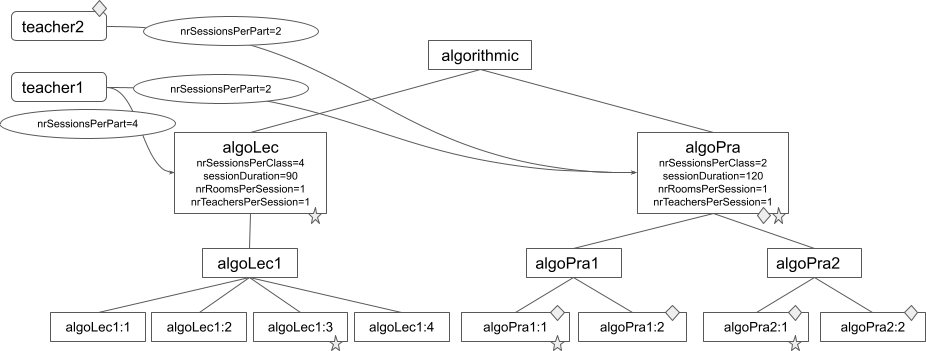
\includegraphics[scale=0.5]{img/utp_rule_1.png}
\caption{Rule interpretation}
\label{fig:utp-rule-1}
\end{figure*}

%\marc{Mettre ici le dernier paragraphe sur la sélection des rangs ? Et l'exemple en fin de section ?}
Let
${\RANK}$
denote the range of session ranks,
${\maptype{\RANK}{\SESSION}}:\RANK\rightarrow2{^\SESSION}$
the rank-based partitioning of sessions,
and
${\LABEL}$
the set of labels 
(${\LABEL}\subseteq2^{{\ENTITY}}$)
completed 
with the whole set of entities to mock label optionality
($\ENTITY\in{\LABEL}$)
and singleton entities to support identity-based selection
($\myset{\myset{e}\ |\ e\in{\ENTITY}}\subseteq{\LABEL}$),
the language of selectors
is the set 
$
\cup_{n\geq1}({\TYPE}\times{\LABEL}\times{2^{\RANK}})^{n}
$.
%where each 
Each selector 
$
d=((T_1,L_1,O_1),\ldots,(T_k,L_k,O_k))
$
%($k\geq1$)
decomposes into a generator
$
(T_1,L_1,O_1)
$
and a possibly empty list of filters
$
((T_2,L_2,O_2),\ldots,(T_k,L_k,O_k))
$.
%A session $s$ is said to satisfy triple
%$
%(T_i,L_i,O_i)
%%\in({\TYPE}\times{\LABEL}\times{2^{\RANK}})
%$
%if
%it is compatible with
%an entity of type $T_i$ and label $L_i$ 
%($s\in\map{T_i}{\SESSION}{L_i}$)\footnote{
%%Let $X\subseteq Y$,
%$
%{\map{Y}{\SESSION}{X}}
%$
%denotes
%$
%\setunion{i}{X\cap Y}{\map{Y}{\SESSION}{i}}
%$.
%}
%and 
%if it satisfies mask $O_i$, i.e., its rank is included in $O_i$
%($s\in\map{\RANK}{\SESSION}{O_i}$).
%A selector 
%$
%d=((T_1,L_1,O_1),\ldots,(T_k,L_k,O_k))
%$
$d$ matches any e-map
whose entity has type $T_1$ and label $L_1$ and whose image includes any compatible session satisfying mask $O_1$ and any of the filters.
The set of e-maps
$\denote{d}$
matched by $d$
%selector 
%$
%d%=
%%((T_1,L_1,O_1),\ldots,(T_k,L_k,O_k))
%$
%represents
%the set of e-maps 
is defined by
\begin{multline*}
\denote{d}=
\bigcup\limits_{e\in{T_1}}
%\myset\left\{(e,S')
\Big \{(e,S')
\ |\ 
%e\in T_1\cap L_1,
S'=
\mape{T_1}{\SESSION}{\myset{e}\cap L_1}
%\cap 
%\map{\RANK}{\SESSION}{O_1}
\;\cap \\
\bigcup\limits_{i=2\ldots k}
{
\mape{T_i}{\SESSION}{L_i}
\cap
\mape{\RANK}{\SESSION}{O_1\cap O_i}
\wedge
S'\neq\emptyset
}
\Big \}
\end{multline*}

where
$
{\mape{X}{Y}{X'}}
=
%$
%denotes
%$
\bigcup\limits_{i\in X'}{\map{X}{Y}{i}}
$
with
$X'\subseteq X$
.

Figure~\ref{fig:utp-rule-1} is a toy example to illustrate the interpretation of rules.
The course \texttt{algorithmic} has 2 parts : lecture part \texttt{algoLec} and practice part \texttt{algoPra}.
There is 1 lecture class, taught by \texttt{teacher1}, and 2 practical classes taught by \texttt{teacher1} and \texttt{teacher2}.
%\todo[inline]{Marc : harmoniser notations}
The lecture class has 4 sessions and each practical class has 2 sessions.
Figure~\ref{fig:utp-rule-1} illustrates the flattening of the following rules: 
%on a simple model consisting of 2 teachers and & course subdivided into 2 parts, 3 classes and 8 sessions. The first rule forbids a time period for 

{\footnotesize{
\begin{multline}
\texttt{\mbox{\hspace*{-1em}}{\FORBIDDENPERIOD}((<(\TEACHER,{teacher2},\_)>,9120,9240)}\label{rule-example-1}\\
\end{multline}
\begin{multline}
\texttt{\mbox{\hspace*{-1em}}{\SEQUENCED}(<(\CLASS,\_,\myset{3}),(\PART,{algoLec},\_)>,}\\
\texttt{<(\CLASS,\_,\myset{1}),(\PART,{algoPra},\_)>)\label{rule-example-2}}
\end{multline}
}}

Rule~\ref{rule-example-1}
requires that \texttt{teacher2} has no session between 8am and 10am the second day of week 2.
In this example, the time grid has 1440 slots a day and 5 days a week, meaning that slot %value\footnote{Each possible session slot is mapped to a single value. All possible values make up the domain of a session.} 
9120 (resp. 9240) corresponds to 8am (resp. 10am) the second day of week 2.
The selector includes no mask and no filter hence matches with all possible sessions of \texttt{teacher2} 
as indicated with diamonds on Figure~\ref{fig:utp-rule-1}. 
The resulting domain of e-maps is the singleton $\myset{(teacher2,\map{\TEACHER}{\SESSION}{teacher2})}$
and the rule is flattened into a single \texttt{\FORBIDDENPERIOD} constraint. %$\myset{\map{\TEACHER}{\SESSION}{teacher2}}$.
Rule~\ref{rule-example-2}
%requires that the first practical session in Algorithmic \todo[inline]{Marc : pourquoi algo ?} start after the third lecture.
requires that the first sessions of the practices start after the third session of the lecture.
The two selectors include a filter. The first selector matches with all class sessions of rank 3 in part \texttt{algoLec}, 
and the second matches with all class sessions of rank 1 in part \texttt{algoPra} as indicated with stars on the figure.
The rule is flattened into 2 \texttt{\SEQUENCED} constraints corresponding to the cross product of the e-map domains $\myset{(algoLec1,\map{\RANK}{\SESSION}{3}\cap\map{\PART}{\SESSION}{algoLec})}$
and $\myset{(algoPra1,\map{\RANK}{\SESSION}{1}\cap\map{\PART}{\SESSION}{algoPra}),(algoPra2,\map{\RANK}{\SESSION}{1}\cap\map{\PART}{\SESSION}{algoPra})}$.

%------------------------------------------------------------
%------------------------------------------------------------
\subsection{Solution}
\label{sec:solution}
The solution component includes assignment decisions
relating to the choice of slots and resources for sessions,
the placement of students in groups and
the assignment of groups to classes.
The solution hence represented may be partial, even empty 
and does not have to be consistent with the built-in constraints or the rules of the instance.
The support for partial solutions allows to tackle subproblems using separate {\UTP} instances and solution seeds.
For instance, a scheduling instance may be defined on the basis of partial and consistent solutions pre-generated for the student sectioning and resource allocation subproblems.
Likewise, the support for inconsistent solutions is paramount to repair solutions that have become inconsistent due to unforeseen changes.

%As mentioned before, 
Student groups are considered a by-product of student sectioning.
For this reason, groups may only be listed in the solution component, not in the entity model, and defined both by the students they include and the classes they are assigned to. 
This sectioning process is subject to different constraints. 
First, students are partitioned into groups and students are inextricably bound to their group.
Second, groups may only include students with identical course registrations.
Third, group-to-class assignments must comply with any subgroup inclusion constraint stated in the entity model.

%Let ${\SLOT}$ denote the range of slots defining the schedule horizon, $\maptype{\PART}{\SLOT}$ denotes the set of allowed slots defined for each course part in the entity model. 
%$\maptype{\SESSION}{\SLOT}$ shall denote the set of slots assigned to each session in a solution component.
%Let ${\GROUP}$ denote the set of groups defined in a solution, $\maptype{\GROUP}{\STUDENT}$ and $\maptype{\CLASS}{\GROUP}$ shall denote respectively the students making up each group and the groups making up each class.



% %The schema thus allows to cast university timetabling problems either as cumulative or disjunctive scheduling problems that subsume student sectioning or not.


% \paragraph{Paragraph headings} Use paragraph headings as needed.
% \begin{equation}
% a^2+b^2=c^2
% \end{equation}

% For one-column wide figures use
%\begin{figure}
% Use the relevant command to insert your figure file.
% For example, with the graphicx package use
%  \includegraphics{example.eps}
% figure caption is below the figure
%\caption{Please write your figure caption here}
%\label{fig:1}       % Give a unique label
%\end{figure}
%
% For two-column wide figures use
%\begin{figure*}
% Use the relevant command to insert your figure file.
% For example, with the graphicx package use
%  \includegraphics[width=0.75\textwidth]{example.eps}
% figure caption is below the figure
%\caption{Please write your figure caption here}
%\label{fig:2}       % Give a unique label
%\end{figure*}
%
% For tables use
%\begin{table}
% table caption is above the table
%\caption{Please write your table caption here}
%\label{tab:1}       % Give a unique label
% For LaTeX tables use
%\begin{tabular}{lll}
%\hline\noalign{\smallskip}
%first & second & third  \\
%\noalign{\smallskip}\hline\noalign{\smallskip}
%number & number & number \\
%number & number & number \\
%\noalign{\smallskip}\hline
%\end{tabular}
%\end{table}




